\chapter{Trees}
In this chapter, we will introduce some fundamental concepts of trees. Trees are hierarchical data structures widely used for various applications such as representing hierarchical relationships, optimizing search operations, and organizing data efficiently. 

\section{General Tree}
\subsection{Nodes}
\begin{minipage}{0.4\textwidth}
A tree is a collection of nodes. The collection can be empty, which is sometimes denoted as \(A\). Otherwise, a tree consists of a distinguished node \(r\), called the root, and zero or more subtrees \(T_1, T_2, \cdots, T_k\), each of whose roots are connected by a directed edge to \(r\). The root of each subtree is said to be a child of \(r\), and \(r\) is the parent of each subtree root.
\end{minipage}
\begin{minipage}{0.6\textwidth}
\begin{figure}[H]
  \centering
  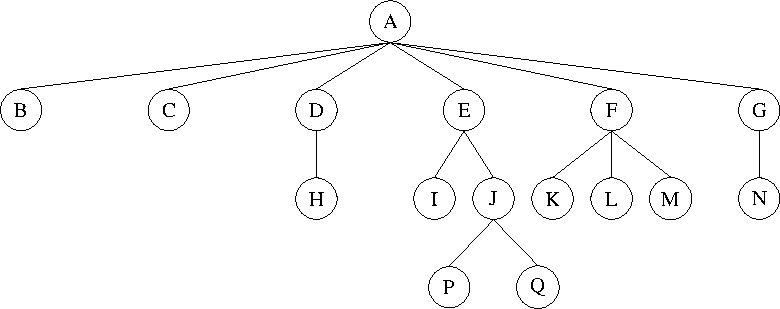
\includegraphics[width=0.8\textwidth]{Figure/General-Tree.pdf}
  \caption{General Tree}
\end{figure}
\end{minipage}

Each node in a tree has a parent and may have an arbitrary number of children, possibly zero. Nodes with no children are known as leaves, and nodes with the same parent are called siblings. For example, in the above graph, \(A\) is the parent of \(D\), and \(B\), \(C\), and \(D\) are siblings.

A path from node \(n_1\) to \(n_k\) is defined as a sequence of nodes \(n_1, n_2, \dots, n_k\) such that \(n_i\) is the parent of \(n_{i+1}\) for \(1 \leq i < k\). The length of this path is the number of edges on the path, namely \(k - 1\). There is a path of length zero from every node to itself, and there is exactly one path from the root to each node.

Also, if there is a path from \(n_1\) to \(n_2\), we call \(n_1\) the ancestor of \(n_2\), while \(n_2\) is the descendant of \(n_1\). If \(n_1 \neq n_2\), we call them a proper ancestor or proper descendant.

For any node \(n_i\), the depth of \(n_i\) is the length of the unique path from the root to \(n_i\). Thus, the root is at depth 0. The height of \(n_i\) is the longest path from \(n_i\) to a leaf. Therefore, all leaves are at height 0. For example, in the graph above, \(E\) is at depth 1 and height 2.

The height of a tree is equal to the height of the root, and the depth of a tree is the depth of the deepest leaf. These two values are always equal, representing the longest path from the root to any leaf.

To implement a tree, we could store both the data and a pointer to each child in the node. However, this approach might not work well for a large number of children. We can solve this issue by keeping the children of each node in a linked list of tree nodes.

\subsection{Traversal}
Suppose we have a directory that includes files and subdirectories. How do we list the names of all the files?

\begin{minipage}{0.6\textwidth}
We can use a technique called tree traversal. To traverse a data structure means to process every node in the data structure exactly once, in whatever way you choose. It is possible to pass the same node multiple times, but it would only be processed once.\\[5pt]
There are three main traversal orders: preorder, inorder, and postorder traversal. However, as long as the traversal follows a systematic way of processing data, it is valid.\\[5pt]
For example, in the graph on the right, we have:\\[5pt]
- Preorder: 013425786  \\[5pt]
- Inorder: 314075826  \\[5pt]
- Postorder: 341785620  \\[5pt]
- Level-order: 012345678
\end{minipage}
\begin{minipage}{0.4\textwidth}
\begin{figure}[H]
  \centering
  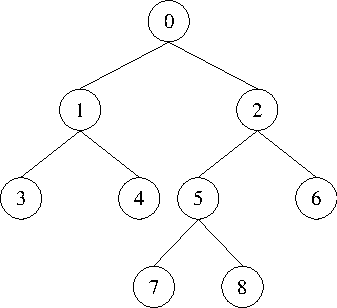
\includegraphics[width=0.8\textwidth]{Figure/Traversal.pdf}
  \caption{Traversal Demonstration}
\end{figure}
\end{minipage}

\section{Binary Tree}
\subsection{Definition}
\begin{minipage}{0.5\textwidth}
  \begin{figure}[H]
    \centering
    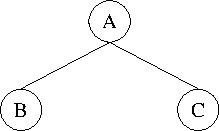
\includegraphics[width=0.5\textwidth]{Figure/Generic-BT.pdf}
    \caption{Generic Binary Tree}
  \end{figure}
\end{minipage}
\begin{minipage}{0.5\textwidth}
  \begin{figure}[H]
    \centering
    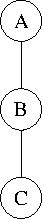
\includegraphics[height=0.3\textwidth]{Figure/Degene-BT.pdf}
    \caption{Degenerated Binary Tree}
  \end{figure}
\end{minipage}

A binary tree is a tree in which no node has more than two children. The depth of an average binary tree is considerably smaller than \(n\). For example, even in the worst case — the degenerate tree — the depth would be \(n - 1\). The average depth is \(O(\frac{h}{2})\), and for a special type of binary tree, namely the binary search tree, the average depth is \(O(\log n)\).

\subsection{Some Binary Trees}
\begin{minipage}{0.5\textwidth}
  \begin{figure}[H]
    \centering
    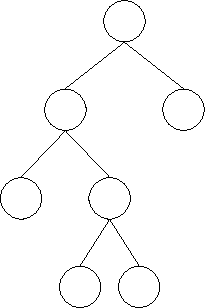
\includegraphics[height=0.3\textwidth]{Figure/FBT.pdf}
    \caption{Full Binary Tree}
  \end{figure}
\end{minipage}
\begin{minipage}{0.5\textwidth}
  \begin{figure}[H]
    \centering
    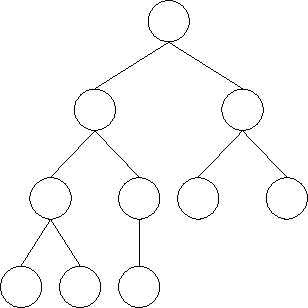
\includegraphics[height=0.3\textwidth]{Figure/CBT.pdf}
    \caption{Complete Binary Tree}
  \end{figure}
\end{minipage}

A full binary tree is a binary tree in which every node, other than the leaves, has exactly two children.

A complete binary tree is a binary tree in which every level, except possibly the last, is completely filled, and all the nodes in the last level are as far left as possible. This means the nodes in the last level are filled from left to right.

\subsection{Implementation}
Since a binary tree has at most two children, we can implement it by keeping direct pointers to them. A node can be represented as an element in a doubly linked list, storing key information along with two pointers to its left and right children. 

We can also implement a node using two pointers: one pointing to its left child and the other pointing to its next sibling.

\section{Expression Tree}
\begin{minipage}{0.6\textwidth}
An expression tree is also a binary tree, which is used to calculate the result of an expression. For example, we can express the expression \(((9 - (2 + 3)) * (7 - 1))\) using the  expression tree on the right.\\[5pt]
In an expression tree, the leaves represent operands, and the internal nodes represent operators. By using inorder traversal, we can recover the original expression. From the binary tree, using postorder traversal, we can obtain the postfix notation. With the use of a stack, we can implement a calculator, as shown in the previous chapter.
\end{minipage}
\begin{minipage}{0.4\textwidth}
\begin{figure}[H]
  \centering
  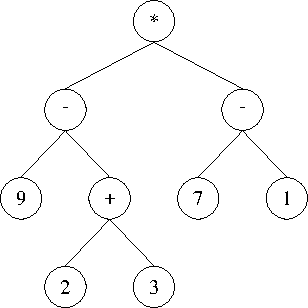
\includegraphics[height=0.6\textwidth]{Figure/Expression-Tree.pdf}
  \caption{Expression Tree}
\end{figure}
\end{minipage}

\section{Binary Search Tree}
\subsection{Definition}
\begin{minipage}{0.6\textwidth}
  A binary search tree (BST) has the same physical property as a binary tree, meaning that nodes have at most two children. However, it also has an ordering property: for each node, all the nodes in its left subtree have smaller values, and all the nodes in its right subtree have larger values. This ordering property turns a binary tree into a binary search tree, and it implies that all the elements in the tree can be ordered in a consistent manner.
\end{minipage}\quad
\begin{minipage}{0.3\textwidth}
  \begin{figure}[H]
    \centering
    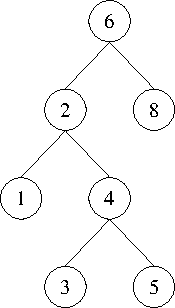
\includegraphics[width=0.4\textwidth]{Figure/BST.pdf}
    \caption{Binary Search Tree}
  \end{figure}
\end{minipage}

\subsection{Operations}
There are some typical operations that can be done on a binary search tree, like make null, find, find max, find min, insertion and deletion. 

For the \verb|Find| operation, it generally requires returning a pointer to the node in tree \(T\) that has key \(x\), or \verb|null| if there is no such node. The structure of the tree makes this simple. If \(T\) is empty, then we can just return \verb|null|. If the key stored at \(T\) is \(x\), we can return \(T\). Otherwise, we make a recursive call on a subtree of \(T\), either left or right, depending on the relationship of \(x\) to the key stored in \(T\).

For the \verb|Find_min| and \verb|Find_max| operations, these routines return the position of the smallest and largest elements in the tree, respectively. To perform \verb|Find_min|, start at the root and go left as long as there is a left child. The stopping point is the smallest element. The \verb|Find_max| routine is the same, except that branching is to the right child.

For insertion, we proceed down the tree. If \(x\) is found, we do nothing (or ``update'' something). Otherwise, we insert \(x\) at the last spot on the path traversed. Duplicates can be handled by keeping an extra field in the node record that indicates the frequency of occurrence.

However, for deletion, it is more difficult since we need to consider several possibilities. If the node is a leaf, it can be deleted immediately. If the node has one child, the node can be deleted after its parent adjusts a pointer to bypass the node. The complicated case is when we need to delete a node with two children. The general idea is to replace the key of the node with the smallest (leftmost) key of the right subtree and recursively delete the node.

\subsection{Analysis}
As mentioned before, the average depth of a binary search tree is \(O(\log n)\). Therefore, intuitively, all operations, except \verb|make_null|, should take \(O(\log n)\) time. The running time of all the operations, except \verb|make_null|, is \(O(d)\), where \(d\) is the depth of the node containing the accessed key. However, how do we get the average depth of \(O(\log n)\)?

\begin{proof}
  Let \(D(n)\) be the internal path length for some tree \(T\) of \(n\) nodes. The internal path length is the sum of the depths of all nodes in a tree, and \(D(1) = 0\). A \(n\)-node tree consists of an \(i\)-node left subtree and an \((n - i - 1)\)-node right subtree, plus a root at depth zero for \(0 \leq i < n\).

  Then we have \(D(i)\) as the internal path length of the left subtree with respect to its root, and we obtain
  \[
    D(n) = D(i) + D(n - i - 1) + n - 1
  \]
  If all subtree sizes are equally likely, which is true for a binary search tree, then the average value of both \(D(i)\) and \(D(n - i - 1)\) is
  \[
    \dfrac{1}{n} \sum_{j = 0}^{n - 1} D(j)
  \]
  Which yields
  \[
    D(n) = \dfrac{2}{n} \left[\sum_{j = 0}^{n - 1} D(j)\right] + n - 1
  \]
\end{proof}

This recurrence gives an average value of \(D(n) = O(n\log n)\). Thus, the expected depth of any node should be \(O(\log n)\).

Another thing to notice is that for the deletion operation, it favors the left subtree. So, after many insertions and deletions, we may end up with an unbalanced binary tree, which would look like a degenerated tree. To ensure that all the nodes can be operated on in \(O(\log n)\) time, we need to make the binary search tree balanced. This is why we have the AVL tree.

\section{AVL Tree}
\subsection{Definition}
\begin{minipage}{0.7\textwidth}
An AVL (Adelson-Velskii and Landis) tree is a binary search tree with a balancing condition. It is identical to a binary search tree, having the same physical and ordering properties. However, for every node in the AVL tree, the heights of the left and right subtrees can differ by at most 1.\\[5pt]
With an AVL tree, all tree operations, except insertion, can be performed in \(O(\log n)\) time.\\[5pt]
To construct the smallest AVL tree of height \(n\), we can use the two smallest AVL subtrees of heights \(n-1\) and \(n-2\). By doing so recursively, we can find the smallest AVL tree.
\end{minipage}
\begin{minipage}{0.3\textwidth}
  \begin{figure}[H]
    \centering
    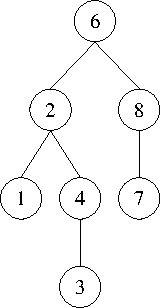
\includegraphics[width=0.4\textwidth]{Figure/AVL.pdf}
    \caption{AVL Tree}
  \end{figure}
\end{minipage}

The height of an empty tree is defined to be \(-1\). Height information is kept for each node. The height of an AVL tree is at most roughly \(1.44\log (n + 2) - 0.328\), but in practice, it is about \(\log (n + 1) + 0.25\).

\subsection{Operations}
All tree operations can be performed in \(O(\log n)\) time, except possibly insertion. Insertion and deletion operations need to update the balancing information since they might violate the AVL tree property. Therefore, we need to restore the property by means of rotations.

A single rotation involves only a few pointer changes and alters the structure of the tree while preserving the search tree property. Rotations happen from the bottom up, meaning we start checking balancing conditions from the lowest affected node and move upward.

For insertion into the right subtree of the right child, we perform a Left Rotation; for insertion into the left subtree of the left child, we perform a Right Rotation. 

\begin{minipage}{0.5\textwidth}
\begin{figure}[H]
  \centering
  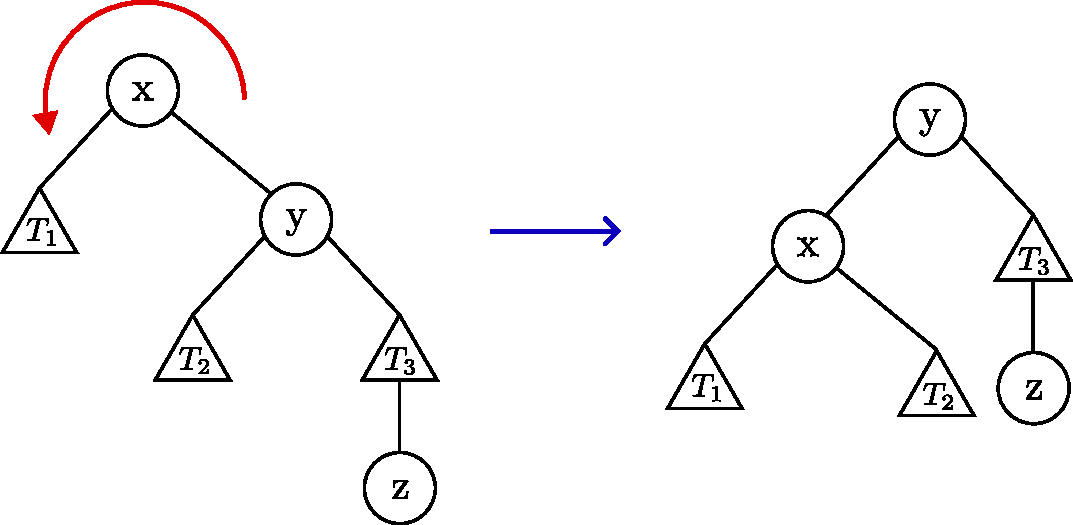
\includegraphics[width=0.8\textwidth]{Figure/RR.pdf}
  \caption{Left Rotation}
\end{figure}
\end{minipage}
\begin{minipage}{0.5\textwidth}
\begin{figure}[H]
  \centering
  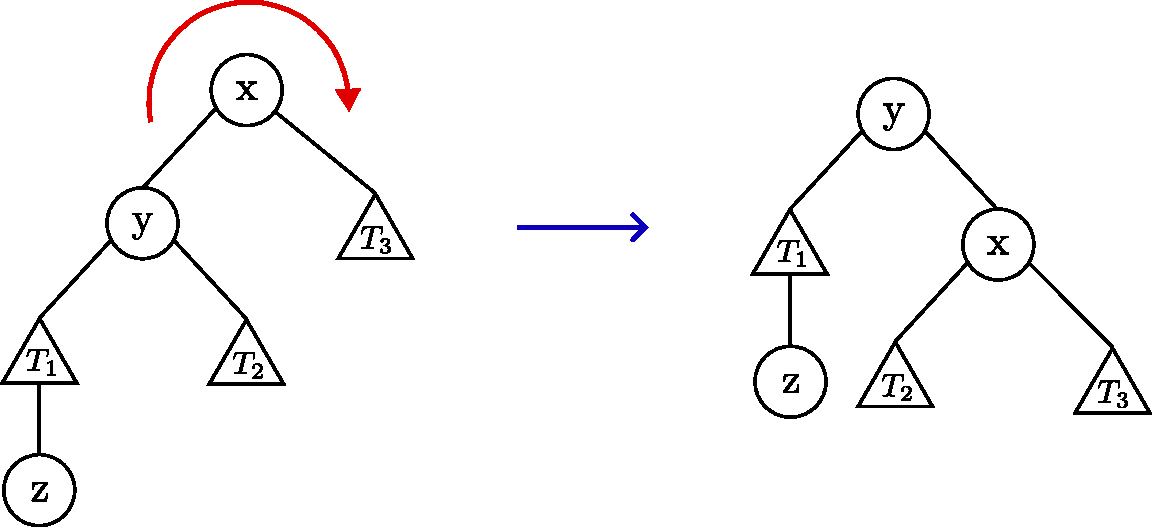
\includegraphics[width=0.8\textwidth]{Figure/LL.pdf}
  \caption{Right Rotation}
\end{figure}
\end{minipage}

However, single rotation might not work for more complex cases, where the height imbalance is caused by a node inserted into the tree containing the middle element, while the other subtrees have identical heights. In such cases, we use a double rotation, which involves four subtrees instead of three.

For insertion into the right subtree of the left child, we use a Left-Right Rotation. For insertion into the left subtree of the right child, we use a Right-Left Rotation. These double rotations help restore balance by first performing a single rotation on the child node and then performing a second rotation on the parent node, ensuring that the AVL tree's balance property is maintained.

\begin{minipage}{0.5\textwidth}
\begin{figure}[H]
  \centering
  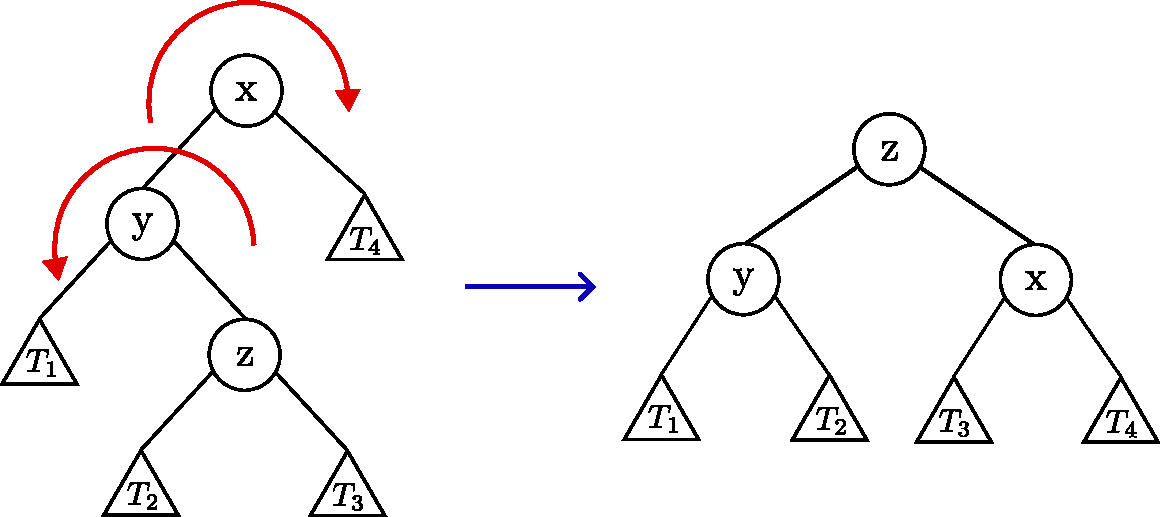
\includegraphics[width=0.8\textwidth]{Figure/LR.pdf}
  \caption{Left-Right Rotation}
\end{figure}
\end{minipage}
\begin{minipage}{0.5\textwidth}
\begin{figure}[H]
  \centering
  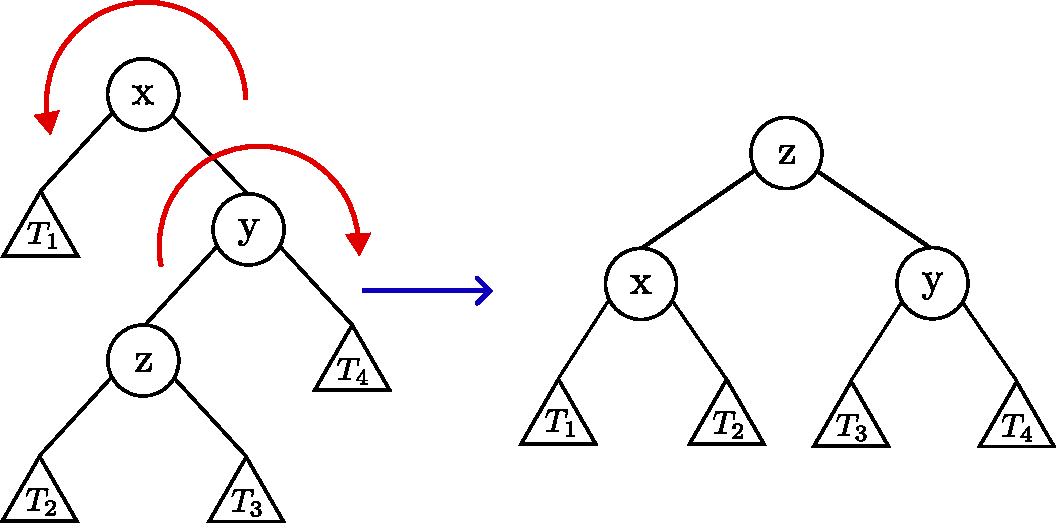
\includegraphics[width=0.8\textwidth]{Figure/RL.pdf}
  \caption{Right-Left Rotation}
\end{figure}
\end{minipage} 

These four rotations help us perform all the necessary balancing operations.

To insert a new node with key \(x\) into an AVL tree \(T\), we recursively insert \(x\) into the appropriate subtree of \(T_{lr}\). If the height of \(T_{lr}\) does not change, then we are done. Otherwise, if a height imbalance occurs, we perform the appropriate single or double rotation depending on \(x\) and the keys in \(T\) and \(T_{lr}\). Finally, we update the height. For example, the method for checking imbalance is demonstrated below:
\begin{figure}[H]
  \centering
  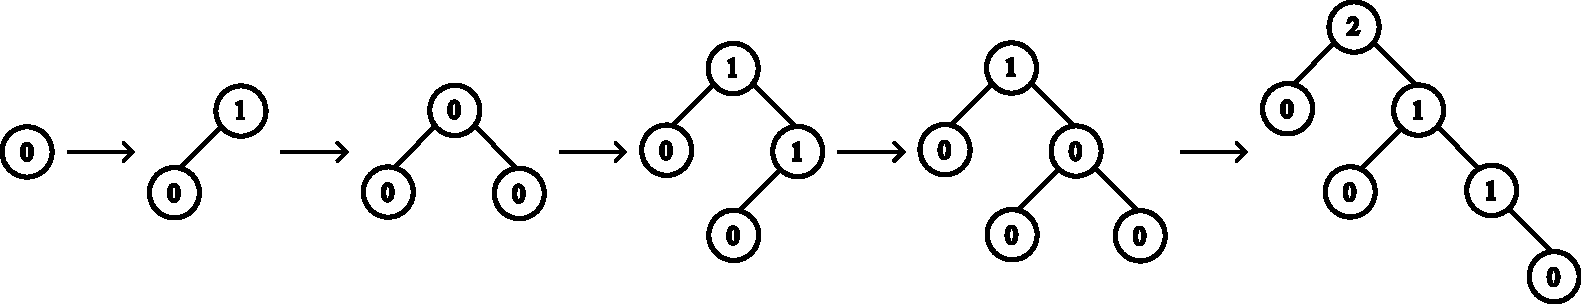
\includegraphics[width=\textwidth]{Figure/AVLInDemo.pdf}
\end{figure}

The implementation of an AVL tree is similar to a binary search tree, with the addition of height information stored in each node. This height information allows the tree to maintain balance by ensuring that the difference in height between the left and right subtrees of any node is at most 1.

\section{B-Tree}
\subsection{Definition}
A B-Tree of order \(m\) is a tree with the following properties:  

- All the leaf nodes must be at the same level (have the same depth).  

- All non-leaf nodes except the root must have at least \(\lceil \frac{m}{2} \rceil - 1\) keys and a maximum of \(m - 1\) keys.  

- All non-leaf nodes except the root (i.e., all internal nodes) must have children between \(\lceil \frac{m}{2} \rceil\) and \(m\).  

- The root is either a leaf or has between 2 and \(m\) children.  

- A non-leaf node with \(n-1\) keys must have \(n\) children.  

- All the key values within a node must be in ascending order.  


\begin{figure}[H]
  \centering
  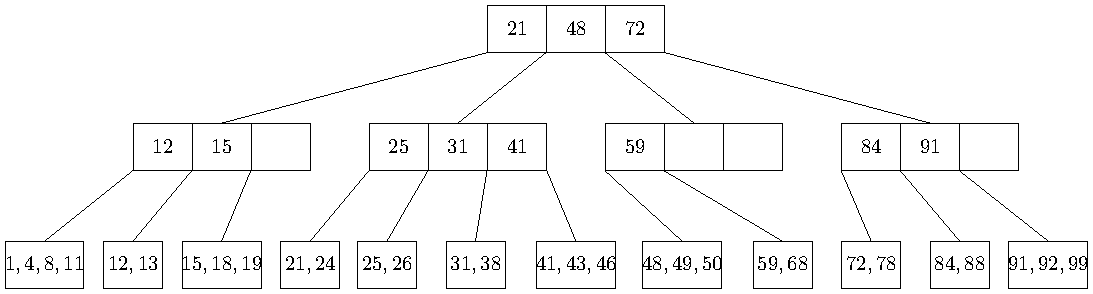
\includegraphics[width=\textwidth]{Figure/B-Tree.pdf}
  \caption{B-tree of order 4}
\end{figure}

A B-tree of order 4 is also known as a 2-3-4 tree; a B-tree of order 3 is also known as a 2-3 tree.

\subsection{Operations}
To insert a key into a node, we need to note the maximum number of values that the node can store. If the node isn't full, we can simply insert the key. However, there are some cases that need to be considered:

To insert 1, we find the location. However, since the leftmost node is full, we cannot insert it there. This can be solved by splitting the node into two nodes with two keys, then adjusting the information of the parent. Next, we try to insert 19. Since the rightmost node is full, we need to split it into two nodes with two children. Then, we continue splitting upwards to the root until we either reach the root node or find a node with fewer than two children.

\begin{minipage}{0.5\textwidth}
\begin{figure}[H]
  \centering
  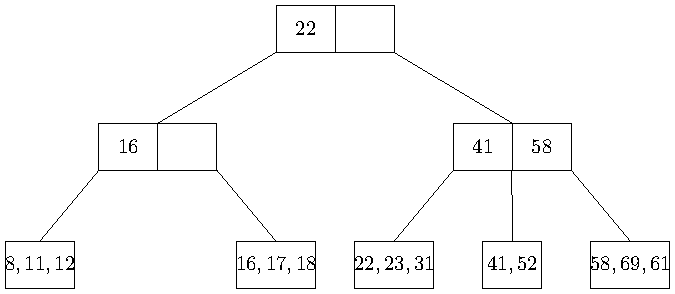
\includegraphics[width=\textwidth]{Figure/BT-23T-D1.pdf}
  \caption{Original Tree}
\end{figure}
\end{minipage}
\begin{minipage}{0.5\textwidth}
\begin{figure}[H]
  \centering
  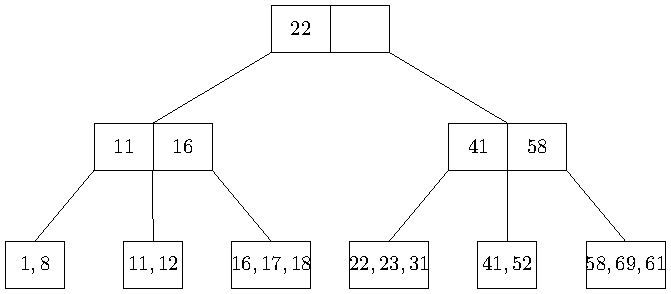
\includegraphics[width=\textwidth]{Figure/BT-23T-D2.pdf}
  \caption{Insert 1}
\end{figure}
\end{minipage}
\begin{figure}[H]
  \centering
  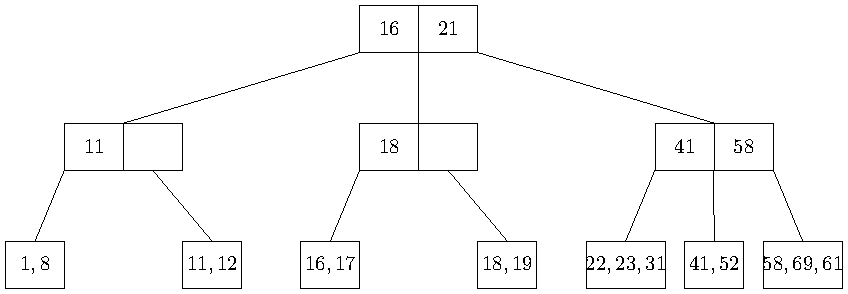
\includegraphics[width=0.7\textwidth]{Figure/BT-23T-D3.pdf}
  \caption{Insert 19}
\end{figure}

The depth of a B-tree is at most \(\lceil \log_{\lceil \frac{m}{2} \rceil} n \rceil\). At each node along the path, we perform \(O(\log m)\) work to determine which branch to take. An insertion or deletion could require \(O(m)\) work to fix up all the information at the node. The worst case for insertion and deletion would be \(O(m \log m n) = O\left(\frac{m}{\log m} \log n\right)\).

In summary, trees are used in operating systems, compiler design, and searching. In practice, all the balanced tree schemes are worse than the simple binary search tree, but this is acceptable.
